% Chapter Template

\chapter{Quantum ergodicity} % Main chapter title

\label{Chapter3} % Change X to a consecutive number; for referencing this chapter elsewhere, use \ref{ChapterX}
\thispagestyle{empty}
%----------------------------------------------------------------------------------------
%	SECTION 1
%----------------------------------------------------------------------------------------

\section{Quantum ergodicity}

Let $(M,g)$ be a compact Riemannian manifold. We recall some general notions from ergodic theory. The time evolution of any classical system on a Riemannian manifold $(M,g)$ is given by the Hamiltonian flow $\Phi^{t}$ on the phase space $T^{\ast}M$ and the flow on each energy shell $\Sigma_{c}=H^{-1}(c)$ simply identifies with the geodesic flow $\vphi^{t}$ on $M$. Hence, the motion occurs on a hypersurface given by $H$. We also recall the definition of Liouville measure \ref{def:Liouville_measure}.\\
It is possible to discuss the ergodicity of the geodesic flow $\Phi_{t}$ by looking at it as a transformation on the measure space $(\Sigma_{c},\mu_{L}^{c})$ and using the discrete definition of ergodicity \ref{definteo:ergodic_discrete}. In fact, if $\vphi^{t}$ is ergodic\footnote{For example, is $M$ has sectional negative curvature.}, then by Birkhoff's theorem \ref{teo:birkhoff} we have
\[
\spn{f}_{T}=\lim_{T\to\infty}\frac{1}{T}\int_{0}^{T}f\Phi_{t}(x))\dd t =\fint_{\Sigma_{c}}f\dd\mu_{L}^{c}.
\]
Moreover, recall the Hamiltonian symbol $\Ham\colon T^{\ast}M\to\R$ given by
\[
\Ham(q,p)\coloneqq\norm{p}^{2}+V(q),
\]
for a smooth potential function $V$, and its (Weyl) quantization $\Xi(\planck)=-\planck^{2}\Lapl+V(x)$, which is the \emph{Schr{\"o}dinger operator}. In particular, $\Op^{W}(\Ham)(x,\planck D)=\Xi(h)$. The following definition will be of frequent use.

\begin{defin}[density of a sequence in a set]
Given a sequence $\{a_{k}\}_{k\geq1}$ of complex numbers, the density of a subsequence $a_{k_{j}}$ is defined by 
\[
\lim_{n\to\infty}\frac{\#\{j\colon k_{j}\leq n\}}{n}.
\] 
We are supposing that the limit does exist.
\end{defin}



We begin our \virg{exploration} of different statements of quantum ergodic theorem by quoting the original result of de Verdière, from 1985, which however in is one of the clearest, in our humble opinion. The statement reads as follows.

\begin{impTeo}{\QE, Schinrelman and de Vérdière, CITA}{QE_original}
% Wong pg50
%\label{teo:QE_original}
Let $M$ be a compact Riemannian manifold. If the geodesic flow on $M$ is ergodic, then there exists a subsequence of eigenvalues $\{\lambda_{k_{i}}\}_{i\in\N}$ of density one of the Laplacian $-\Lapl$ such that, for any pseudodifferential operator $A$ of order zero with principal symbol $a$, it holds
\[
\lim_{i\to \infty}\pscl{A\vphi_{k_{i}}}{\vphi_{k_{i}}}=\int_{\sigma_{c}}a \dd\mu^{c}_{L}, 
\]
where $\vphi_{k_{i}}$ is a Laplacian's eigenfunction for the eigenvalue $\lambda_{k_{i}}$.
\end{impTeo}

In light of this theorem, it is pretty obvious why negatively-curved Riemannian manifolds are of main interest in this topic: by Hopf's theorem \ref{teo:Hopf_theorem}, the geodesic flow on those manifolds is ergodic and, hence, theorem \ref{impTeo:QE_original} holds.\\

An immediate consequence of this theorem is the following.

\begin{cor}
\label{cor:liouville_density}
Keeping the notation of theorem \ref{impTeo:QE_original} and letting $A$ be a open subset of $M$, we have
\[
\lim_{i\to\infty}\int_{A}\abs{\vphi_{k_{i}}}^{2}=\frac{\Vol(A)}{\Vol(M)}.
\]
\end{cor}

Now several remarks follow.

\begin{remark}
\begin{itemize}
\item The quantity $\pscl{A\vphi_{n}}{\vphi_{n}}$ represents the expectation value of the self-adjont operator $A$. So, from this perspective, theorem \ref{impTeo:QE_original} states that the expectation value of a quantum observable is just the space-average of its corresponding classical symbol.
\item The statement of the theorem can be revised in the sense of measure convergence; in fact, the theorem essentialy states that the induced-measures sequence converge to the uniform distribution in the weak$^{\star}$-sense.
\item We can give a more striking physical interpretation of theorem \ref{impTeo:QE_original}. In fact, wavefunctions on a negatively-curved compact domain equidistribute in the high-energy limit. If the classical part of a system, i.e. the geodesic flow, is ergodic, then even in the semiclassical limit $\planck_{n}\to0$ (or $\lambda_{n}\to\infty$) do most eigenfunctions not localize in the phase space.
\end{itemize}
\end{remark}

We will present a more general statement than theorem \ref{impTeo:QE_original}, involving not only operator $\Lapl$, but also the more general Schr{\"o}dinger operator $\Xi(\planck)$, to be consistent with the general framework of semiclassical analysis. To introduce the general theorem \ref{teo:QE_Zeld_zwors}, we need the following definition.

\begin{defin}[Uniform symbol]
Let $a$ be a symbol and let $A=\Op^{w}(a)(q,\planck\Diff)$. Then $a$ is \emph{uniform} if for all $t\in[a,b]$,
\[
\alpha\coloneqq\fint_{\Sigma_{t}}\sigma(A)\dd\mu_{L}
\]
is constant with respect to $t$, i.e. the averages of $a$ over energy-shells $\Ham^{-1}(c)$ are all equal to some $\alpha$. A $\PDO$ is uniform if its principal symbol is.
\end{defin}

It should be noted that any symbol $b$ can be made uniform, via the application of the correct pojection to the set of uniform symbols. This projection $\Pi$ can be defined in the following way. We refer to METTI ZWORKSI for further details. Assuming that $\norm{\partial\Ham}>\alpha>0$ on $\Ham^{-1}([a,b])$, we can assure ourselves that $\norm{\partial\Ham}>\alpha/2$ on $\Ham^{-1}[a-\veps,b+\veps]$ for a sufficient small positive parameter $\veps>0$. If $d=\Ham(x,p)$ then we define
\[
\Pi\left(b(x,p)\right)\coloneqq b(x,p)-\fint_{\Sigma_{d}}b\dd\mu_{L}^{d}
\]
for every symbol $b$. In particular, we have
\[
\fint_{\Ham^{-1}(c)}\Pi(b)\dd\mu_{L}^{c}=0,\quad\forall c\in[a,b].
\]
Using a \emph{bump function} $\chi\in C_{c}^{\infty}(\Ham^{-1}((a-\veps,b+\veps))$ such that it is equal to $1$ on $\Ham^{-1}([a,b])$, it is possible to define $\Pi$ on manifolds $M$ as 
\[
\Pi\colon C^{\infty}(T^{\ast}M)\to C_{c}^{\infty}(T^{\ast}M),\quad \Pi(b)=
\]
In particular, it can be proved, using the equality $\fint_{\Ham^{-1}(d)}\Pi(b)\dd\mu^{d}_{L}=0$, that $\Pi$ is indeed a projection, i.e. is idempotent. The previous equality $\fint_{\Ham^{-1}(c)}\Pi(b)\dd\mu^{c}_{L}=0$ holds for any choice of the symbol $b$. Thus, $\Pi$ maps arbitrary symbols to uniform symbols of zero average.\\

The next theorem is a version of the celebrated \QE theorem for operator $\Xi(\planck)$.

\begin{nteo}[\QE, Zelditch and Zworski]
\label{teo:QE_Zeld_zwors}
Let $(M,g)$ be a compact Riemannian manifold with ergodic geodesic flow. If $A\in\Psi(M)$ is uniform, with principal symbol $\sigma(A)$, then 
\[
(2\pi\planck)^{n}\sum_{a\leq \lambda_{k}\leq b}\abs{
\pscl{A\vphi_{k}}{\vphi_{k}}-\fint_{\{a\leq\Ham(x,p)\leq b}\sigma(A)\dd x\dd p
}^{2}\to0,
\]
for $\planck\to0$ and $\forall\lambda_{k}$ eigenvalues of $\Xi(\planck)$ in the interval $[a,b]$, with corrispondent eigenfuncions $\vphi_{k}$.
\end{nteo}

This theorem can be slightly modified to consider the case $\planck=1$ and $\Xi(\planck)=-\Lapl$, implying theorem \ref{impTeo:QE_original}.


\begin{nese}[equidistribution of $\Lapl$-eigenfunctions]
\label{ese:equidis}
Let $(M,g)$ be a Riemannian manifold such that the geodesic flow is ergodic. Let $\Lapl=\Lapl_{g}$ the Laplacian operator on $M$, with respect to the metric $g$.\\
Theorem \ref{impTeo:QE_original} assures us that there is a subsequence $k_{i}\to\infty$ of density $1$ such that 
\[
\int_{M}\abs{\vphi_{k_{i}}^{2}}f\dd x \rightarrow\int_{M}f\dd x.
\]
\end{nese}


This general framework basically sets up the starting point of \emph{quantum unique ergodicity}:\\[2mm]
\textit{
Under the hypothesis of theorem \ref{teo:QE_Zeld_zwors} or \ref{impTeo:QE_original}, do these probability measures induced by eigenfunctions always converge to the uniform measures?
}

We approach this point in the next section.



\section{Quantum unique ergodicity}

\label{sec:que_intro}


We will start from a brief heuristic reasoning. The quantum ergodicity theorem gives an answer regarding the asymptotic evolution of Laplacian eigenfunctions, in case of classical ergodicity. In particular, \QE theorems examine the quantities $\pscl{A\vphi_{k}}{\vphi_{k}}$, where $A$ is a semiclassical $\PDO$, corrisponding to principal symbol $\sigma(A)=a$. Mathematically and physically, these quantities are the most obvious to consider in the asymptotic limit, because their analytical expression is most certainly impossible to write down. In this sense, these quantities gives birth, in a natural way, to sort of \virg{eigenfunction-induced} measure, the \emph{\textbf{Wigner measures}}. The Wigner measure (mentioned in chapter \ref{Chapter05}) of the state $\vphi_{k}$ on $T^{\ast}M$ is defined by
\begin{equation}
\label{eq:def_wigner_measure}
\mu_{k}(a)\coloneqq\pscl{A\vphi_{k}}{\vphi_{k}}.
\end{equation}
In fact, the projection of one of this measure to the manifold $M$ is equal to the probability measure $\lambda_{k}\coloneqq\abs{\vphi_{k}(x)}^{2}\dd x$ and for this reason the measure $\mu_{k}$ is called \emph{\textbf{microlocal lift}} of measure $\lambda_{k}^{M}$. As measures on the phase space $T^{\ast}M$, $\mu_{k}$ also carries with itself informations about the functions $\vphi_{k}$.

\begin{defin}
\label{def:Wigner_measure}
Let $A\in\Psi(M)$ has principal symbol $a=\sigma(A)$. Then, the measure on $T^{\ast}M$ defined by
\[
\mu(a(x,p))=\pscl{A\vphi_{k}}{\vphi_{k}}
\]
is called Wigner measure of eigenfunction $\vphi_{k}$ for $\Xi(\planck)$. The transformation of measures from $M$ to $T^{\ast}M$ defined by
\[
\mu_{k}=\abs{\vphi_{k}}^{2}\dd x\mapsto\pscl{A\vphi_{k}}{\vphi_{k}}=\mu_{k}
\]
is called \emph{microlocal lift}.
\end{defin}

Usually, it is an hopeless task to analysize the Wigner measure for a given eigenfunction $\vphi_{k}$. However, again, we could shift our interest to the asymptotic behaviour of this measures. The following definition is fundamental to make more rigourous the concept of \virg{asymptotic behaviour} for measures.

\begin{defin}
\label{def:weak_convergence_star}
A sequence of measures $\{\mu_{k}\}_{k\geq0}$ on a manifold $M$ converges to a measure $\mu$ in the weak-$\ast$ topology if 
\[
\lim_{k\to\infty}\int f\dd\mu_{k}=\int f\dd\mu,\quad\forall f\in C^{\infty}_{c}(M)
\]
\end{defin}

\begin{defin}[Quantum limit]
\label{def:quantum_limit_measure}
A weak-$ast$ limit $\mu$ of a subsequence of Wigner measures is called \textbf{quantum limit measure}.
\end{defin}

We will take for granted that any quantum limit $\mu$ possesses the following two properties:
\begin{compactitem}
\item $\mu$ is a probability measure on any given energy shell $\sigma_{c}$.
\item $\mu$ is invariant with respect to the geodesic flow $\Phi_{t}$ on $M$.
\end{compactitem} 

In particular, the second statement can derived directly from Egorov's theorem \ref{impTeo:egorov}. Setting the stage for introducing the definition of \QUE, we now rewrite the definition of \QE as follows.
\begin{defin}
\label{def:new_def_qe}
If $M$ is a compact Riemannian manifold with ergodic geodesic flow, then there exists a subsequence $\{\vphi_{k_{j}}\}_{j\geq0}$ of eigenfunctions of density $1$ such that the Wigner measures satisfy $\mu_{k_{j}}\to\mu_{L}^{c}$ on $\Sigma_{c}$ for $j\to\infty$. 
\end{defin}

The point is the uniqueness of Liouville measure as the only possible quantum limit.


In this way, it is possible to view that \QUE is much stronger than \QE: equidistribution occur not only on the configuration manifold $M$, but also on the energy surface $\Sigma_{c}$.\\

If \QUE fails, it means that there are some subsequence of Wigner measures, that could be very very sparse among all eigenvalues, that have a different quantum limit, reflecting some particular behaviour of the underlying classical system. The general and most famous conjecture in this field is due to Zeev Rudnick and Peter Sarnak, first formulated in 1993 \cite{RudSarn:conj}. It reads as follows.

\begin{impConj}{Rudnick, Sarnak}{conj_rudn_sarn}
If $(M,g)$ is a Riemannian manifold with negative curvature, then the sequence of Wigner measures $\mu_{k}$ induced by eigenfunctions of operator $\Xi(\planck)$ converges to the Liouville measure $\mu_{L}^{c}$ on any energy shell $\Sigma_{c}=\Ham^{-1}(c)$.
\end{impConj}

A reason behind the difficulty to tackle \QUE with respect to \QE is that \QUE deals with not only with convergence of
measures, but also with the elimination of all possible exceptional eigenfunctions. In particular, this aspect defy standard semiclassical tools, as Weyl's law. In fact, it should be necessary to have a control not only on one sequence of eigenfunction, but on every possible sequence.\\

To present both sides of \QUE (when it holds and when it does not), in the next section we briefly present how Hassell managed to prove that \QUE fails for the Bunimovich Stadium $\BS_{l}$. On the other hand, in the chapter \ref{Chapter5}, we will present a major result of E. Lindenstrauss, which essentially ensures that \QUE hold for hyperbolic surface with an additional arithmetical structure.



%-----------------------------------
%	SUBSECTION 1
%-----------------------------------
\section{Hassell disproof of \QUE}



The $\BS_{l}$ billiard has a different behaviour from the geodesic flow on negative curved surfaces, as it can be seen from figure in chapter \ref{Chapter05}. Indeed, both of them are ergodic and mixing systems, but the rectuangular part of $\BS_{l}$ gives birth to some interesting, nonetheless trivial, periodic orbits: it is the one-parameter family of orbits that corrisponds to billiards bouncing back and forth vertically against the horizontal walls.
This situation is called \emph{bouncing ball mode} and the phenomenon of \emph{scarring} involving these modes was studied by Heller as early as 1984. In this sense, this phenomenon gives a heuristical reason for the failure of \QUE in $\BS_{l}$ case. The motion in the $\BS$ is still \QE, as those trivial periodic orbits form a set of (Liouville) measure zero, but \QUE fails as this regime is still present in the high-eigenvalue limit. (In figure \ref{fig:bunimov_eigenstates} it is possible to see 4 of this \virg{bouncing-modes})
\begin{figure}[h]
\centering
  %

    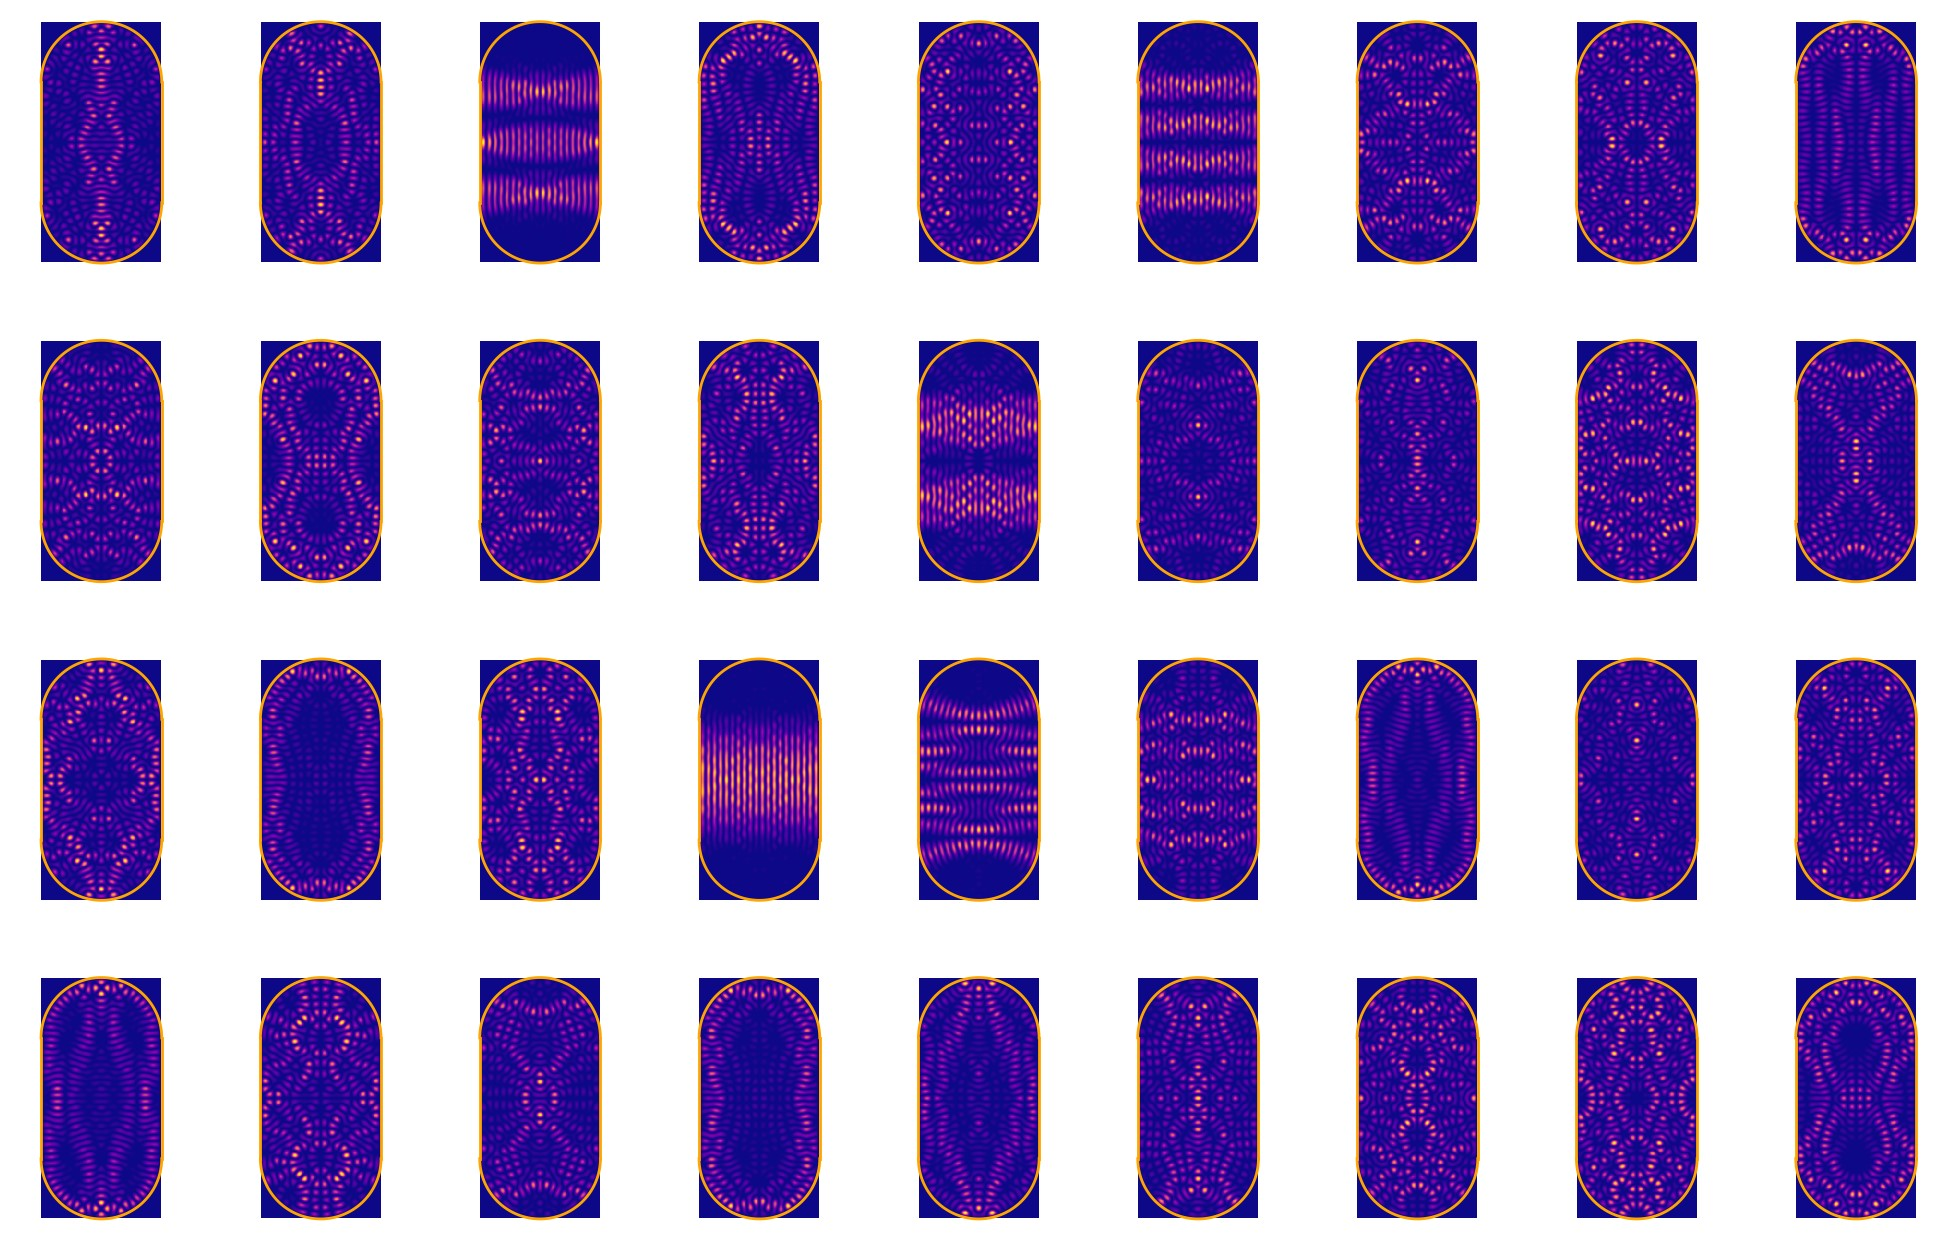
\includegraphics[scale=0.32,angle=0]{quant_stad_neig36_level1000_4per9.jpg}

    \noindent\\
  \decoRule
  \caption{Bunimovich stadium 36 eigenfunctions, for $\lambda\sim1000$}
  \label{fig:bunimov_eigenstates}
\end{figure}

 In fact, Hassell's main result (\cite{Hass:billiards_not}) shows that some high-eigenvalue eigenstates of $\BS_{l}$ do indeed have a positive mass on the bouncing ball orbits.

\begin{impTeo}{Hassell}{hassell_stadium}
For every $\veps>0$, there exist a subset $B_{\veps}\subset[1,2]$ of measure at least $1-4\veps$ and a constant $m(\veps)>0$ with the following property: for every $l\in B_{\veps}$, there exist a quantum limit formed from Dirichlet eigenfunctions of $\Lapl$ on the $\BS_{l}$ that gives probability mass at least $m(\veps)$ to the bouncing ball trajectories.
\end{impTeo}


The result of Hassell was foreshadow by numerical computations (see also chapter \ref{Chapter6}) and is based on construction of \emph{quasi-modes}, approximate solutions for
eigenfuctions given by Wentzel-Kramers-Brillouin (WKB) methods. The main obstacle in reaching the proof was to show that \virg{bouncing-ball} eigenfunctions (i.e. the corrispondent wigner measures) exist in the high-energy limit. Hassell's proof is a combination of the following techniques:


\begin{compactitem}
\item the \emph{Heller-Zelditch argument}, mettere referenza:\\ 
this method shows that eigenfunctions of $\Lapl$ localize on any Bunimovich stadium $\BS_{t}$, with the (possible) exception of eigenvalues lying in intervals of the form $[n^{2}-O(1),n^{2}+O(1)]$, with $n\in\N$. It can be proved that, if there really only $O(1)$ eigenvalues in this intervall, then eigenfunctions can localize, i.e. \virg{scarring} can occur in momentum space for these intervals (see Tao \cite{tao:site}). Reaching this bound ($O(1)$) is the difficult part of this step; 
\item the \emph{Hadamard variation formula}:\\
one of the main difficulties in approaching the previous task is the fact that Weyl's law has too large error term to get the desired bound. Hassell used this formula, which shows how the eigenvalues of $\BS_{l}$ vary with the aspect ratio of its rectangular component $t$. The formula is given by
\[
\frac{\dd }{\dd l}\lambda_{k}(l)=-\int_{\partial\BS_{l}}\frac{\sgn(x)}{2}(Y\cdot\overrightarrow{n})\abs{\partial_{\overrightarrow{n}}\vphi_{k}(x,l)}^{2}\dd s,
\]
where $(\vphi_{k},\lambda_{k})$ is an eigenvector-eigenvalue pair of the Laplacian $\Lapl$ with Dirichlet boundary condition on $\BS_{l}$, $\overrightarrow{n}$ is the outward unit normal vector at $\partial\BS_{l}$ and $\dd s$ is \virg{curvilinear element} on $\partial\BS_{t}$. Since $\sgn(x)/2(\partial_{x}\cdot\overrightarrow{n})\geq0$ always, the formula shows that, as $t$ increases, the magnitude of $\lambda_{k}$ decreases instead, for fixed $k$. One should not be surprised by this, because Weyl's law gives us 
\[
\lambda_{k}=\frac{4\pi k}{\Area(\BS_{t})}(1+o(1))
\]
and we see that $t$ and $\lambda_{k}$ are \virg{almost inversely proportional}. Using this formula, Hassell shows the refinement
\[
-\frac{\dd}{\dd l}\lambda_{k}(l)\sim \lambda_{k}(l)
\]
in expectation over $k$.
\item \emph{quantum unique ergodicity}:\\
this is used to reach a contradiction. More explicity, if $\BS_{l}$ is \QUE, then by Egorov's theorem \ref{impTeo:egorov} essentially positions and momenta of eigenfunctions in $T^{\ast}\BS_{l}$ are driven by the geodesic flow. At this point, Hassell uses this general argument (\cite{tao:site},\cite{Hass:billiards_not}): in classical dynamics, all geodesic in $\BS_{t}$ eventually interesect its boundary, and it can be shown that for any equidistributed eigenfunction, its normal derivative is also equidistributed on $\partial\BS_{l}$; hence, all eigenfunctions are equidistributed on $\partial\BS_{l}$ and this would imply that the exponential decay, given by Hadamard formula, holds for every $\lambda_{k}$, and not just in expectation. If this would be the case, it could be shown besides that the $\Lapl$-eigenvalues cannot concentrate in interval of the form $[n^{2}-O(1),n^{2}+O(1)]$ for most $l\in [1,2]$, else the eigenvalues would lay around $n^{2}$ for intervals of $t$ of measure non-zero, getting a contradiction with the exponential decay. The Heller-Zelditch argument then gives a contradiction to \QUE assumption.
\end{compactitem}


\begin{remark}
\label{remark:unique_non_que_bun_std}
It is important to highlight that the Bunimovich Stadium $\BS_{l}$ is the only known dynamical billiard for which we have a complete understanding of \QE and \QUE to date. In particular, it is the only one for which we know that \QUE does not hold. On the contrary, there many other systems, like the cardioid stadium $\CS$ and Barnett stadium are believed to be \QUE.
\end{remark}


METTERE FIGURA CARDIOIDE AUTOFUNZIONI?


%\subsection{Quantum maps}
%
%Cita MARKLOFF
%
%It is oftentimes useful to extend the ergodicity of the geodesic flow to the ergodicity of any map on the sympletic phase space $T^{\ast}M$, where $(M,g)$ is a Riemannian manifold. The dynamics on this system can be provided by a discrete map 
%
%
%An explicit and one of the most famous example of this subject is given by \emph{Arnold's cat map}, defined by the action of the map
%\[
%\Sigma=\Matrix{1&1\\1&2}
%\]
%on the 2-dimensional torus $\T^{2}$. In coordinates, for $(q,p)\in \R^{2}\setminus\Z^{2}$, we have $(x,y)\mapsto(q+p,q+2p)\mod1$. Without going in details, altough it has been shown that analogue of \QUE for hyperbolic toral automorphisms (properly speaking, symplectomorphisms) fails to hold (this does not contradicts remark \ref{remark:unique_non_que_bun_std}, as this system is not related to billiards). This suggests that may be something unique about the geodesic flow on a negatively curved manifold. 



%METTI FIGURA AZIONE MAPPA ARNOLD


